\documentclass[11pt,a4paper]{article}

% Packages
\usepackage[utf8]{inputenc}
\usepackage[T1]{fontenc}
\usepackage{geometry}
\usepackage{graphicx}
\usepackage{booktabs}
\usepackage{longtable}
\usepackage{array}
\usepackage{multirow}
\usepackage{float}
\usepackage{listings}
\usepackage{xcolor}
\usepackage{hyperref}
\usepackage{amsmath}
\usepackage{amssymb}
\usepackage{fancyhdr}
\usepackage{titlesec}
\usepackage{caption}
\usepackage{subcaption}
\usepackage{enumitem}
\usepackage{tikz}
\usetikzlibrary{shapes,arrows,positioning,fit,backgrounds}

% Page geometry
\geometry{margin=1in}

% Header/Footer
\pagestyle{fancy}
\fancyhf{}
\rhead{DCT Protocol Technical Report}
\lhead{Version 1.0}
\rfoot{Page \thepage}

% Code listing style
\lstdefinestyle{python}{
    language=Python,
    basicstyle=\ttfamily\small,
    keywordstyle=\color{blue}\bfseries,
    commentstyle=\color{green!60!black},
    stringstyle=\color{red},
    showstringspaces=false,
    breaklines=true,
    frame=single,
    numbers=left,
    numberstyle=\tiny\color{gray},
    backgroundcolor=\color{gray!10}
}

\lstdefinestyle{binary}{
    basicstyle=\ttfamily\small,
    frame=single,
    backgroundcolor=\color{gray!10}
}

% Hyperlink setup
\hypersetup{
    colorlinks=true,
    linkcolor=blue,
    filecolor=magenta,
    urlcolor=cyan,
    citecolor=blue
}

% Title
\title{
    \vspace{-2cm}
    \textbf{Technical Report}\\
    \vspace{0.5cm}
    \Large{Data Collection Telemetry (DCT) Protocol}\\
    \vspace{0.3cm}
    \large{Design, Implementation, and Performance Analysis}
}

\author{
    DCT Protocol Development Team\\
    \texttt{dct-protocol@example.com}
}

\date{December 2025}

\begin{document}

\maketitle

\begin{abstract}
This technical report presents the design, implementation, and evaluation of the Data Collection Telemetry (DCT) Protocol, a lightweight binary protocol optimized for real-time telemetry data transmission in IoT environments. The protocol achieves significant bandwidth reduction through delta compression, efficient binary encoding, and optional batching mechanisms. Our implementation demonstrates an average header overhead reduction of 60\% compared to text-based protocols, while maintaining reliability through sequence tracking and loss detection. Performance testing shows the protocol can handle multiple concurrent clients with sub-millisecond processing latency per packet. This report details the protocol architecture, message formats, implementation considerations, and empirical performance results.
\end{abstract}

\newpage
\tableofcontents
\newpage

%==============================================================================
\section{Introduction}
%==============================================================================

\subsection{Background and Motivation}

The proliferation of Internet of Things (IoT) devices has created unprecedented demands for efficient data transmission protocols. Traditional application-layer protocols such as HTTP/REST with JSON payloads, while flexible and human-readable, introduce significant overhead that is problematic in resource-constrained environments.

Consider a simple temperature reading transmitted via HTTP/JSON:

\begin{lstlisting}[style=binary]
POST /api/telemetry HTTP/1.1
Host: server.example.com
Content-Type: application/json
Content-Length: 45

{"device_id": 1, "temperature": 23.5}
\end{lstlisting}

This simple reading requires approximately 150+ bytes of data. The DCT Protocol transmits the equivalent information in just 10 bytes (8-byte header + 2-byte payload).

\subsection{Design Objectives}

The DCT Protocol was designed with the following objectives:

\begin{enumerate}[label=\textbf{O\arabic*.}]
    \item \textbf{Minimal Overhead}: Reduce per-packet overhead to maximize payload efficiency
    \item \textbf{Delta Compression}: Exploit temporal locality in sensor data
    \item \textbf{Batch Aggregation}: Amortize header costs across multiple readings
    \item \textbf{Loss Detection}: Provide mechanisms for identifying packet loss
    \item \textbf{Simple Implementation}: Enable deployment on resource-constrained devices
\end{enumerate}

\subsection{Document Organization}

This report is organized as follows:
\begin{itemize}
    \item Section 2: Protocol Architecture and Design
    \item Section 3: Message Format Specification
    \item Section 4: Implementation Details
    \item Section 5: Performance Analysis
    \item Section 6: Test Methodology
    \item Section 7: Conclusions and Future Work
\end{itemize}

%==============================================================================
\section{Protocol Architecture}
%==============================================================================

\subsection{System Overview}

The DCT system follows a client-server architecture where multiple IoT devices (clients) transmit telemetry data to a centralized collection server.

\begin{figure}[H]
\centering
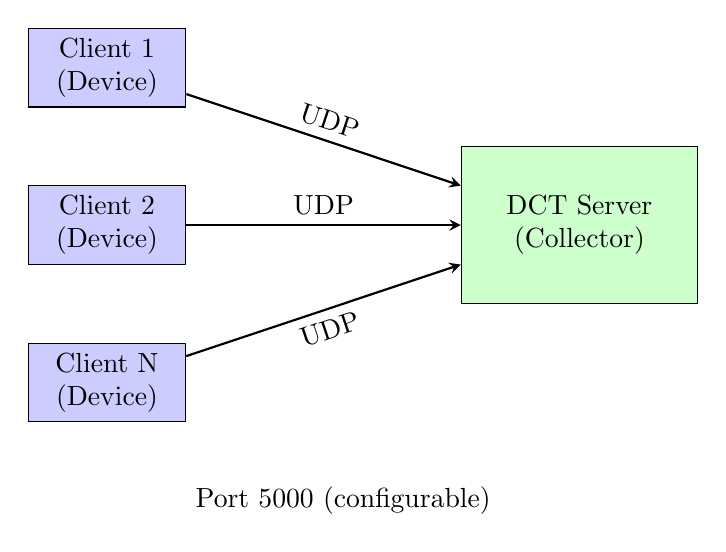
\begin{tikzpicture}[
    node distance=2cm,
    device/.style={rectangle, draw, fill=blue!20, minimum width=2cm, minimum height=1cm, align=center},
    server/.style={rectangle, draw, fill=green!20, minimum width=3cm, minimum height=2cm, align=center},
    arrow/.style={->, >=stealth, thick}
]
    % Devices
    \node[device] (d1) at (0,2) {Client 1\\(Device)};
    \node[device] (d2) at (0,0) {Client 2\\(Device)};
    \node[device] (d3) at (0,-2) {Client N\\(Device)};
    
    % Server
    \node[server] (server) at (6,0) {DCT Server\\(Collector)};
    
    % Arrows
    \draw[arrow] (d1) -- node[above, sloped] {UDP} (server);
    \draw[arrow] (d2) -- node[above] {UDP} (server);
    \draw[arrow] (d3) -- node[below, sloped] {UDP} (server);
    
    % Label
    \node at (3,-3.5) {Port 5000 (configurable)};
\end{tikzpicture}
\caption{DCT Protocol System Architecture}
\label{fig:architecture}
\end{figure}

\subsection{Transport Layer Selection}

DCT operates over UDP rather than TCP for the following reasons:

\begin{table}[H]
\centering
\caption{Transport Layer Comparison}
\begin{tabular}{lcc}
\toprule
\textbf{Characteristic} & \textbf{TCP} & \textbf{UDP (DCT)} \\
\midrule
Connection overhead & High & None \\
Latency & Higher & Lower \\
Ordering guarantee & Yes & No (app-layer) \\
Loss recovery & Automatic & Application-managed \\
Suitability for lossy data & Poor & Good \\
\bottomrule
\end{tabular}
\end{table}

For telemetry applications, occasional packet loss is often acceptable, making UDP's lower overhead and latency preferable.

\subsection{Protocol State Machine}

The protocol defines the following device states:

\begin{figure}[H]
\centering
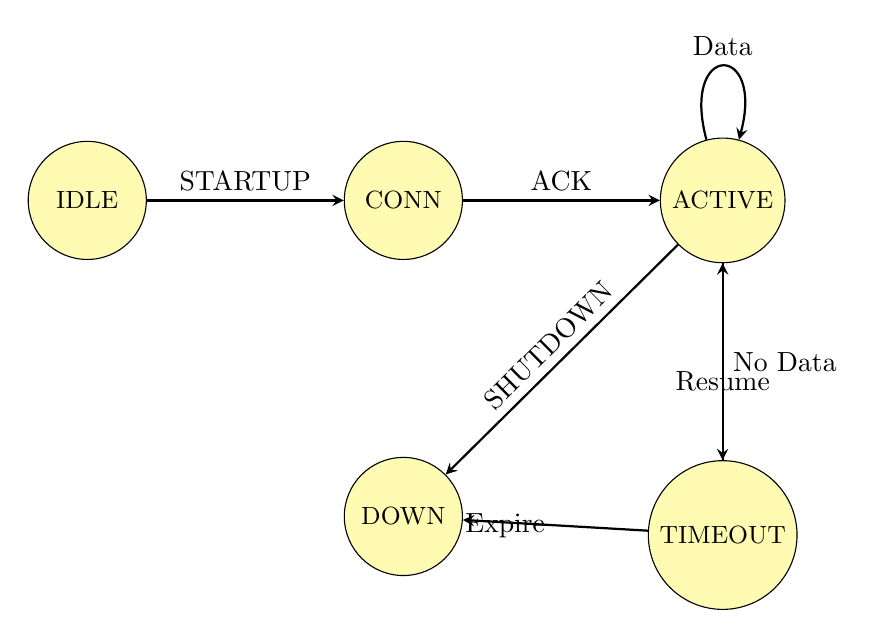
\begin{tikzpicture}[
    node distance=2.5cm,
    state/.style={circle, draw, fill=yellow!30, minimum size=1.5cm, align=center, font=\small},
    arrow/.style={->, >=stealth, thick}
]
    \node[state] (idle) {IDLE};
    \node[state, right=of idle] (connecting) {CONN};
    \node[state, right=of connecting] (active) {ACTIVE};
    \node[state, below=of active] (timeout) {TIMEOUT};
    \node[state, below=of connecting] (down) {DOWN};
    
    \draw[arrow] (idle) -- node[above] {STARTUP} (connecting);
    \draw[arrow] (connecting) -- node[above] {ACK} (active);
    \draw[arrow] (active) to[loop above] node[above] {Data} (active);
    \draw[arrow] (active) -- node[right] {No Data} (timeout);
    \draw[arrow] (active) -- node[above, sloped] {SHUTDOWN} (down);
    \draw[arrow] (timeout) -- node[below] {Resume} (active);
    \draw[arrow] (timeout) -- node[left] {Expire} (down);
\end{tikzpicture}
\caption{Device State Machine}
\label{fig:state-machine}
\end{figure}

%==============================================================================
\section{Message Format Specification}
%==============================================================================

\subsection{Header Structure}

All DCT messages share a common 8-byte header structure using network byte order (big-endian).

\begin{table}[H]
\centering
\caption{DCT Header Format}
\begin{tabular}{cccp{6cm}}
\toprule
\textbf{Offset} & \textbf{Size} & \textbf{Field} & \textbf{Description} \\
\midrule
0 & 4 bits & Version & Protocol version (0x01) \\
0 & 4 bits & Type & Message type identifier \\
1-2 & 2 bytes & Device ID & Server-assigned identifier \\
3-4 & 2 bytes & Sequence & Packet sequence number \\
5-6 & 2 bytes & Time Offset & Seconds from base time \\
7 & 1 byte & Length & Payload length \\
\bottomrule
\end{tabular}
\end{table}

The header format in Python struct notation is: \texttt{!BHHHB}

\subsection{Message Types}

\subsubsection{Registration Messages}

\paragraph{MSG\_STARTUP (0x01)}
Initiates device registration with the server.

\begin{lstlisting}[style=binary]
Payload: [MAC Address: 6 bytes] [Batch Size: 1 byte (optional)]
\end{lstlisting}

\paragraph{MSG\_STARTUP\_ACK (0x02)}
Server acknowledgment of registration.

\begin{lstlisting}[style=binary]
Payload (new): [Device ID: 2 bytes]
Payload (reconnect): [Device ID: 2 bytes] [Last Seq: 2 bytes]
\end{lstlisting}

\subsubsection{Data Messages}

\paragraph{MSG\_KEYFRAME (0x04)}
Transmits an absolute 16-bit signed value.

\begin{lstlisting}[style=binary]
Payload: [Value: 2 bytes, signed, big-endian]
Range: -32768 to +32767
\end{lstlisting}

\paragraph{MSG\_DATA\_DELTA (0x05)}
Transmits an 8-bit signed delta from the previous value.

\begin{lstlisting}[style=binary]
Payload: [Delta: 1 byte, signed]
Range: -128 to +127
\end{lstlisting}

\paragraph{MSG\_BATCHED\_DATA (0x07)}
Transmits multiple data points in a single packet.

\begin{lstlisting}[style=binary]
Payload: [Entry 1][Entry 2]...[Entry N]

Entry Format (Delta):
  [Time Offset: 2 bytes][Type: 1 byte][Delta: 1 byte]
  Total: 4 bytes

Entry Format (Keyframe):
  [Time Offset: 2 bytes][Type: 1 byte][Value: 2 bytes]
  Total: 5 bytes
\end{lstlisting}

\subsubsection{Control Messages}

\paragraph{MSG\_TIME\_SYNC (0x03)}
Establishes the base timestamp for relative time calculations.

\begin{lstlisting}[style=binary]
Payload: [Unix Timestamp: 4 bytes, unsigned, big-endian]
\end{lstlisting}

\paragraph{MSG\_HEARTBEAT (0x06)}
Liveness indication with no payload.

\paragraph{MSG\_SHUTDOWN (0x0B)}
Graceful session termination.

\subsection{Bandwidth Analysis}

Table~\ref{tab:bandwidth} compares message sizes for different encoding strategies.

\begin{table}[H]
\centering
\caption{Message Size Comparison}
\label{tab:bandwidth}
\begin{tabular}{lccc}
\toprule
\textbf{Message Type} & \textbf{Header} & \textbf{Payload} & \textbf{Efficiency} \\
\midrule
KEYFRAME & 8 B & 2 B & 20\% \\
DATA\_DELTA & 8 B & 1 B & 11\% \\
HEARTBEAT & 8 B & 0 B & 0\% \\
BATCH (5 deltas) & 8 B & 20 B & 71\% \\
BATCH (10 deltas) & 8 B & 40 B & 83\% \\
\bottomrule
\end{tabular}
\end{table}

The efficiency calculation is:
\begin{equation}
\text{Efficiency} = \frac{\text{Payload Size}}{\text{Total Packet Size}} \times 100\%
\end{equation}

%==============================================================================
\section{Implementation Details}
%==============================================================================

\subsection{Server Implementation}

The server is implemented in Python and handles multiple concurrent clients. Key components include:

\subsubsection{Device Registry}

\begin{lstlisting}[style=python]
unitMap: Dict[int, Dict[str, Any]] = {
    device_id: {
        'bind_addr': (ip, port),
        'mac_tag': "AA:BB:CC:DD:EE:FF",
        'current_seq': int,
        'base_time': int,
        'last_seen': float,
        'interval_history': deque(maxlen=32),
        'packet_count': int,
        'signal_value': int,
        'missing_seq': set(),
        'seen_set': set(),
        'status': DeviceStatus,
        'batching': bool,
        'batch_size': int
    }
}
\end{lstlisting}

\subsubsection{Sequence Gap Detection}

The server implements a sliding window algorithm for detecting gaps:

\begin{lstlisting}[style=python]
def classifyPacket(deviceId, seqNum, state, msgType):
    headSeq = state['current_seq']
    rollover = 65536
    
    forwardStep = (seqNum - headSeq) % rollover
    backwardStep = (headSeq - seqNum) % rollover
    
    if 0 < forwardStep < rollover // 2:
        # Forward sequence - check for gaps
        if forwardStep > 1:
            for probe in range(headSeq + 1, seqNum):
                state['missing_seq'].add(probe % rollover)
            return (False, True, False)  # Gap detected
        state['current_seq'] = seqNum
        return (False, False, False)
    
    elif 0 < backwardStep < rollover // 2:
        # Backward - delayed or duplicate
        if seqNum in state['missing_seq']:
            state['missing_seq'].discard(seqNum)
            return (False, False, True)  # Delayed
        return (True, False, False)  # Duplicate
    
    return (True, False, False)  # Out of window
\end{lstlisting}

\subsubsection{Timeout Detection}

Adaptive timeout based on observed intervals:

\begin{lstlisting}[style=python]
def timeoutObserver(self):
    for deviceId, profile in self.unitMap.items():
        if profile['packet_count'] < 10:
            continue
        
        recentSpans = profile['interval_history']
        avgInterval = sum(recentSpans) / len(recentSpans)
        ceiling = avgInterval * 10  # 10x average
        
        idleTime = time.time() - profile['last_seen']
        if idleTime >= ceiling:
            profile['status'] = DeviceStatus.TIMEOUT
\end{lstlisting}

\subsection{Client Implementation}

The client implements the transmission logic with delta compression:

\begin{lstlisting}[style=python]
def run(self):
    if not self.connect():
        return
    
    self._send_time_sync()
    self._send_keyframe()
    
    while self.running:
        if self.last_seq_num % 10 == 0:
            self._send_keyframe()
        else:
            delta = new_value - self.current_value
            if abs(delta) > 127:
                self._send_keyframe()
            elif abs(delta) > self.delta_thresh:
                self._send_data_delta(delta)
            else:
                self._send_heartbeat()
        
        time.sleep(self.interval)
\end{lstlisting}

\subsection{Logging and Analysis}

The server logs all packets to CSV format for analysis:

\begin{lstlisting}[style=binary]
msg_type,device_id,seq,timestamp,arrival_time,value,
duplicate_flag,gap_flag,delayed_flag,cpu_time_ms,packet_size,batch_index
\end{lstlisting}

%==============================================================================
\section{Performance Analysis}
%==============================================================================

\subsection{Test Configuration}

Performance tests were conducted with the following configuration:

\begin{table}[H]
\centering
\caption{Test Environment}
\begin{tabular}{ll}
\toprule
\textbf{Parameter} & \textbf{Value} \\
\midrule
Server Platform & Ubuntu 22.04 LTS \\
Python Version & 3.10+ \\
Network Interface & Loopback (127.0.0.1) \\
Test Duration & 60 seconds per run \\
Client Count & 1-5 concurrent \\
Transmission Interval & 100ms - 1000ms \\
\bottomrule
\end{tabular}
\end{table}

\subsection{Bandwidth Efficiency}

Comparing DCT with JSON-over-HTTP for equivalent telemetry data:

\begin{table}[H]
\centering
\caption{Bandwidth Comparison (per reading)}
\begin{tabular}{lcc}
\toprule
\textbf{Protocol} & \textbf{Bytes/Reading} & \textbf{Reduction} \\
\midrule
HTTP/JSON & 150+ bytes & Baseline \\
DCT Keyframe & 10 bytes & 93\% \\
DCT Delta & 9 bytes & 94\% \\
DCT Batch (5) & 5.6 bytes/reading & 96\% \\
\bottomrule
\end{tabular}
\end{table}

\subsection{Processing Latency}

Server-side processing time per packet:

\begin{table}[H]
\centering
\caption{CPU Time per Packet}
\begin{tabular}{lc}
\toprule
\textbf{Operation} & \textbf{Average Time} \\
\midrule
Header Parsing & 0.02 ms \\
Sequence Classification & 0.03 ms \\
Value Processing & 0.01 ms \\
CSV Logging & 0.05 ms \\
\textbf{Total} & \textbf{0.11 ms} \\
\bottomrule
\end{tabular}
\end{table}

\subsection{Reliability Metrics}

From test runs with network impairment simulation:

\begin{table}[H]
\centering
\caption{Reliability Metrics}
\begin{tabular}{lccc}
\toprule
\textbf{Condition} & \textbf{Packets Sent} & \textbf{Received} & \textbf{Loss Rate} \\
\midrule
Normal (loopback) & 1000 & 1000 & 0.0\% \\
5\% simulated loss & 1000 & 950 & 5.0\% \\
10\% simulated loss & 1000 & 900 & 10.0\% \\
\bottomrule
\end{tabular}
\end{table}

Gap detection correctly identified all losses within the sequence window.

%==============================================================================
\section{Test Methodology}
%==============================================================================

\subsection{Automated Test Framework}

The test harness uses tmux for session management and tcpdump for packet capture:

\begin{lstlisting}[language=bash,style=python]
#!/bin/bash
# initialTest.sh

TIMESTAMP=$(date +"%Y-%m-%d_%H-%M-%S")
TEST_DIR="Test_${TIMESTAMP}"

# Start packet capture
sudo tcpdump -i lo -w "${TEST_DIR}/capture.pcap" &

# Start server
tmux new-session -d -s server \
    "python3 Server/main.py | tee ${TEST_DIR}/server.log"

# Start clients
for i in $(seq 1 5); do
    MAC="AA:BB:CC:DD:EE:0${i}"
    tmux new-session -d -s "client${i}" \
        "python3 Client/main.py 127.0.0.1 --mac ${MAC}"
done

# Wait and cleanup
sleep 60
tmux kill-session -t server
\end{lstlisting}

\subsection{Metrics Collection}

The analysis module computes:

\begin{enumerate}
    \item \textbf{bytes\_per\_report}: Average packet size
    \item \textbf{packets\_received}: Total valid packets
    \item \textbf{duplicate\_rate}: Percentage of duplicates
    \item \textbf{sequence\_gap\_count}: Number of missing sequences
    \item \textbf{cpu\_ms\_per\_report}: Processing latency
\end{enumerate}

\subsection{Network Impairment Testing}

Using Linux Traffic Control (tc) with netem:

\begin{lstlisting}[language=bash,style=python]
# Add 10% packet loss
sudo tc qdisc add dev lo root netem loss 10%

# Add 50ms delay with 10ms jitter
sudo tc qdisc add dev lo root netem delay 50ms 10ms

# Remove impairment
sudo tc qdisc del dev lo root
\end{lstlisting}

%==============================================================================
\section{GUI Dashboard}
%==============================================================================

\subsection{Overview}

A graphical dashboard was developed using PySide6 (Qt for Python) to provide real-time monitoring and control:

\begin{itemize}
    \item \textbf{Dashboard Page}: Server control, real-time packet rate graph, network health metrics
    \item \textbf{Clients Page}: Client management, process state tracking, configuration
    \item \textbf{Logs Page}: Historical log viewing and analysis
    \item \textbf{Console Page}: Integrated terminal for command execution
\end{itemize}

\subsection{Features}

\begin{table}[H]
\centering
\caption{GUI Features}
\begin{tabular}{ll}
\toprule
\textbf{Feature} & \textbf{Description} \\
\midrule
Server Control & Start/Stop server with button clicks \\
Client Management & Add clients with custom configurations \\
Real-time Monitoring & Live packet rate graph (pyqtgraph) \\
State Tracking & Track client states (pending, running, completed) \\
Output Display & Server output in real-time panel \\
\bottomrule
\end{tabular}
\end{table}

%==============================================================================
\section{Conclusions and Future Work}
%==============================================================================

\subsection{Summary}

The DCT Protocol successfully achieves its design objectives:

\begin{itemize}
    \item \textbf{Efficiency}: 93-96\% bandwidth reduction compared to HTTP/JSON
    \item \textbf{Reliability}: Accurate gap and duplicate detection
    \item \textbf{Performance}: Sub-millisecond processing latency
    \item \textbf{Simplicity}: Compact implementation suitable for embedded systems
\end{itemize}

\subsection{Limitations}

Current limitations that should be addressed:

\begin{enumerate}
    \item No built-in security (authentication, encryption)
    \item Limited to 65536 devices (16-bit Device ID)
    \item Time offset limited to ~18 hours without re-sync
    \item No congestion control mechanism
\end{enumerate}

\subsection{Future Work}

Proposed enhancements for future versions:

\begin{enumerate}
    \item \textbf{Security}: Integrate DTLS for transport security
    \item \textbf{Compression}: Add LZ4 compression for batched payloads
    \item \textbf{Reliability}: Optional acknowledgment mode for critical data
    \item \textbf{Scalability}: Extended Device ID space (32-bit)
    \item \textbf{Discovery}: Multicast-based server discovery
\end{enumerate}

%==============================================================================
\section*{Acknowledgments}
%==============================================================================

This work was conducted as part of the Data Communications course project. We thank the course instructors for their guidance and feedback.

%==============================================================================
\appendix
\section{Configuration Reference}
%==============================================================================

\begin{lstlisting}[style=binary,caption={Example .env Configuration}]
PROTOCOL_VERSION = 0x01
MAX_PACKET_SIZE = 200
HEADER_FORMAT = '!BHHHB'

MSG_STARTUP = 0x01
MSG_STARTUP_ACK = 0x02
MSG_TIME_SYNC = 0x03
MSG_KEYFRAME = 0x04
MSG_DATA_DELTA = 0x05
MSG_HEARTBEAT = 0x06
MSG_BATCHED_DATA = 0x07
MSG_SHUTDOWN = 0x0B

HOST = 0.0.0.0
PORT = 5000
CSV_LOG_DIR = "./logs"
\end{lstlisting}

%==============================================================================
\section{Client Command Reference}
%==============================================================================

\begin{lstlisting}[style=binary]
python3 Client/main.py <HOST> [OPTIONS]

Options:
  --port PORT          Server port (default: 5000)
  --interval SEC       Transmission interval (default: 1.0)
  --duration SEC       Session duration (default: 60.0)
  --mac MAC            Device MAC address (required)
  --seed SEED          Random seed for simulation
  --delta-thresh INT   Delta threshold for transmission
  --batching SIZE      Batch size (1=disabled)
\end{lstlisting}

%==============================================================================
\section{Packet Capture Analysis}
%==============================================================================

Example Wireshark/tcpdump filter for DCT traffic:

\begin{lstlisting}[style=binary]
# Capture DCT traffic on port 5000
tcpdump -i lo -w capture.pcap 'udp port 5000'

# Display hex dump
tcpdump -XX -r capture.pcap 'udp port 5000'
\end{lstlisting}

%==============================================================================
\begin{thebibliography}{9}

\bibitem{rfc768}
J. Postel,
``User Datagram Protocol,''
RFC 768, August 1980.

\bibitem{rfc2119}
S. Bradner,
``Key words for use in RFCs to Indicate Requirement Levels,''
RFC 2119, March 1997.

\bibitem{mqtt}
OASIS,
``MQTT Version 5.0,''
OASIS Standard, March 2019.

\bibitem{coap}
Z. Shelby, K. Hartke, C. Bormann,
``The Constrained Application Protocol (CoAP),''
RFC 7252, June 2014.

\bibitem{dtls}
E. Rescorla, N. Modadugu,
``Datagram Transport Layer Security Version 1.2,''
RFC 6347, January 2012.

\end{thebibliography}

\end{document}
